\documentclass[11pt,a4paper]{article}
\usepackage[utf8]{inputenc}
\usepackage[margin=1in]{geometry}
\usepackage{amsmath}
\usepackage{amssymb}
\usepackage{graphicx}
\usepackage{hyperref}
\usepackage{listings}
\usepackage{xcolor}
\usepackage{booktabs}
\usepackage{float}

% Python code styling
\lstset{
    language=Python,
    basicstyle=\ttfamily\small,
    keywordstyle=\color{blue},
    commentstyle=\color{gray},
    stringstyle=\color{red},
    showstringspaces=false,
    breaklines=true,
    frame=single,
    backgroundcolor=\color{gray!10}
}

\title{Machine Learning Assignment 2}
\author{Dataset ID: 23-23--23}
\date{}

\begin{document}

\maketitle

\begin{center}
Name: Sayan Mondal\\
Student ID: 24377372\\
Strand: Future Networked Systems\\
Course: MSc. Computer Science
\end{center}
    
\vspace{1em}

\subsection*{(i)(a)}

To begin, I imported the data set and visualized it in 3D to get a sense of what the data looked like. The data set contains 199 observations with two input features ($x_1$, $x_2$) and one target variable ($y$).

\begin{lstlisting}
import numpy as np
import matplotlib.pyplot as plt
from mpl_toolkits.mplot3d import Axes3D

data = np.loadtxt('week3.csv', delimiter=',', skiprows=1)
X = data[:, :2]
y = data[:, 2]

fig = plt.figure()
ax = fig.add_subplot(111, projection='3d')

# plot points colored by target value
scatter = ax.scatter(X[:,0], X[:,1], y, c=y, cmap='viridis', s=30)

ax.set_xlabel('Feature 1 (x1)')
ax.set_ylabel('Feature 2 (x2)')
ax.set_zlabel('Target (y)')
ax.set_title('3D Scatter Plot')

# add colorbar
plt.colorbar(scatter, ax=ax, shrink=0.5, aspect=5, label='Target (y)')

plt.show()
\end{lstlisting}

The points are colored by their target value using the viridis colormap where the dark colors represent lower $y$ values and brighter colors represent higher $y$ values. This color coding helps visualize how the target changes across the feature space.

\begin{figure}[H]
\centering
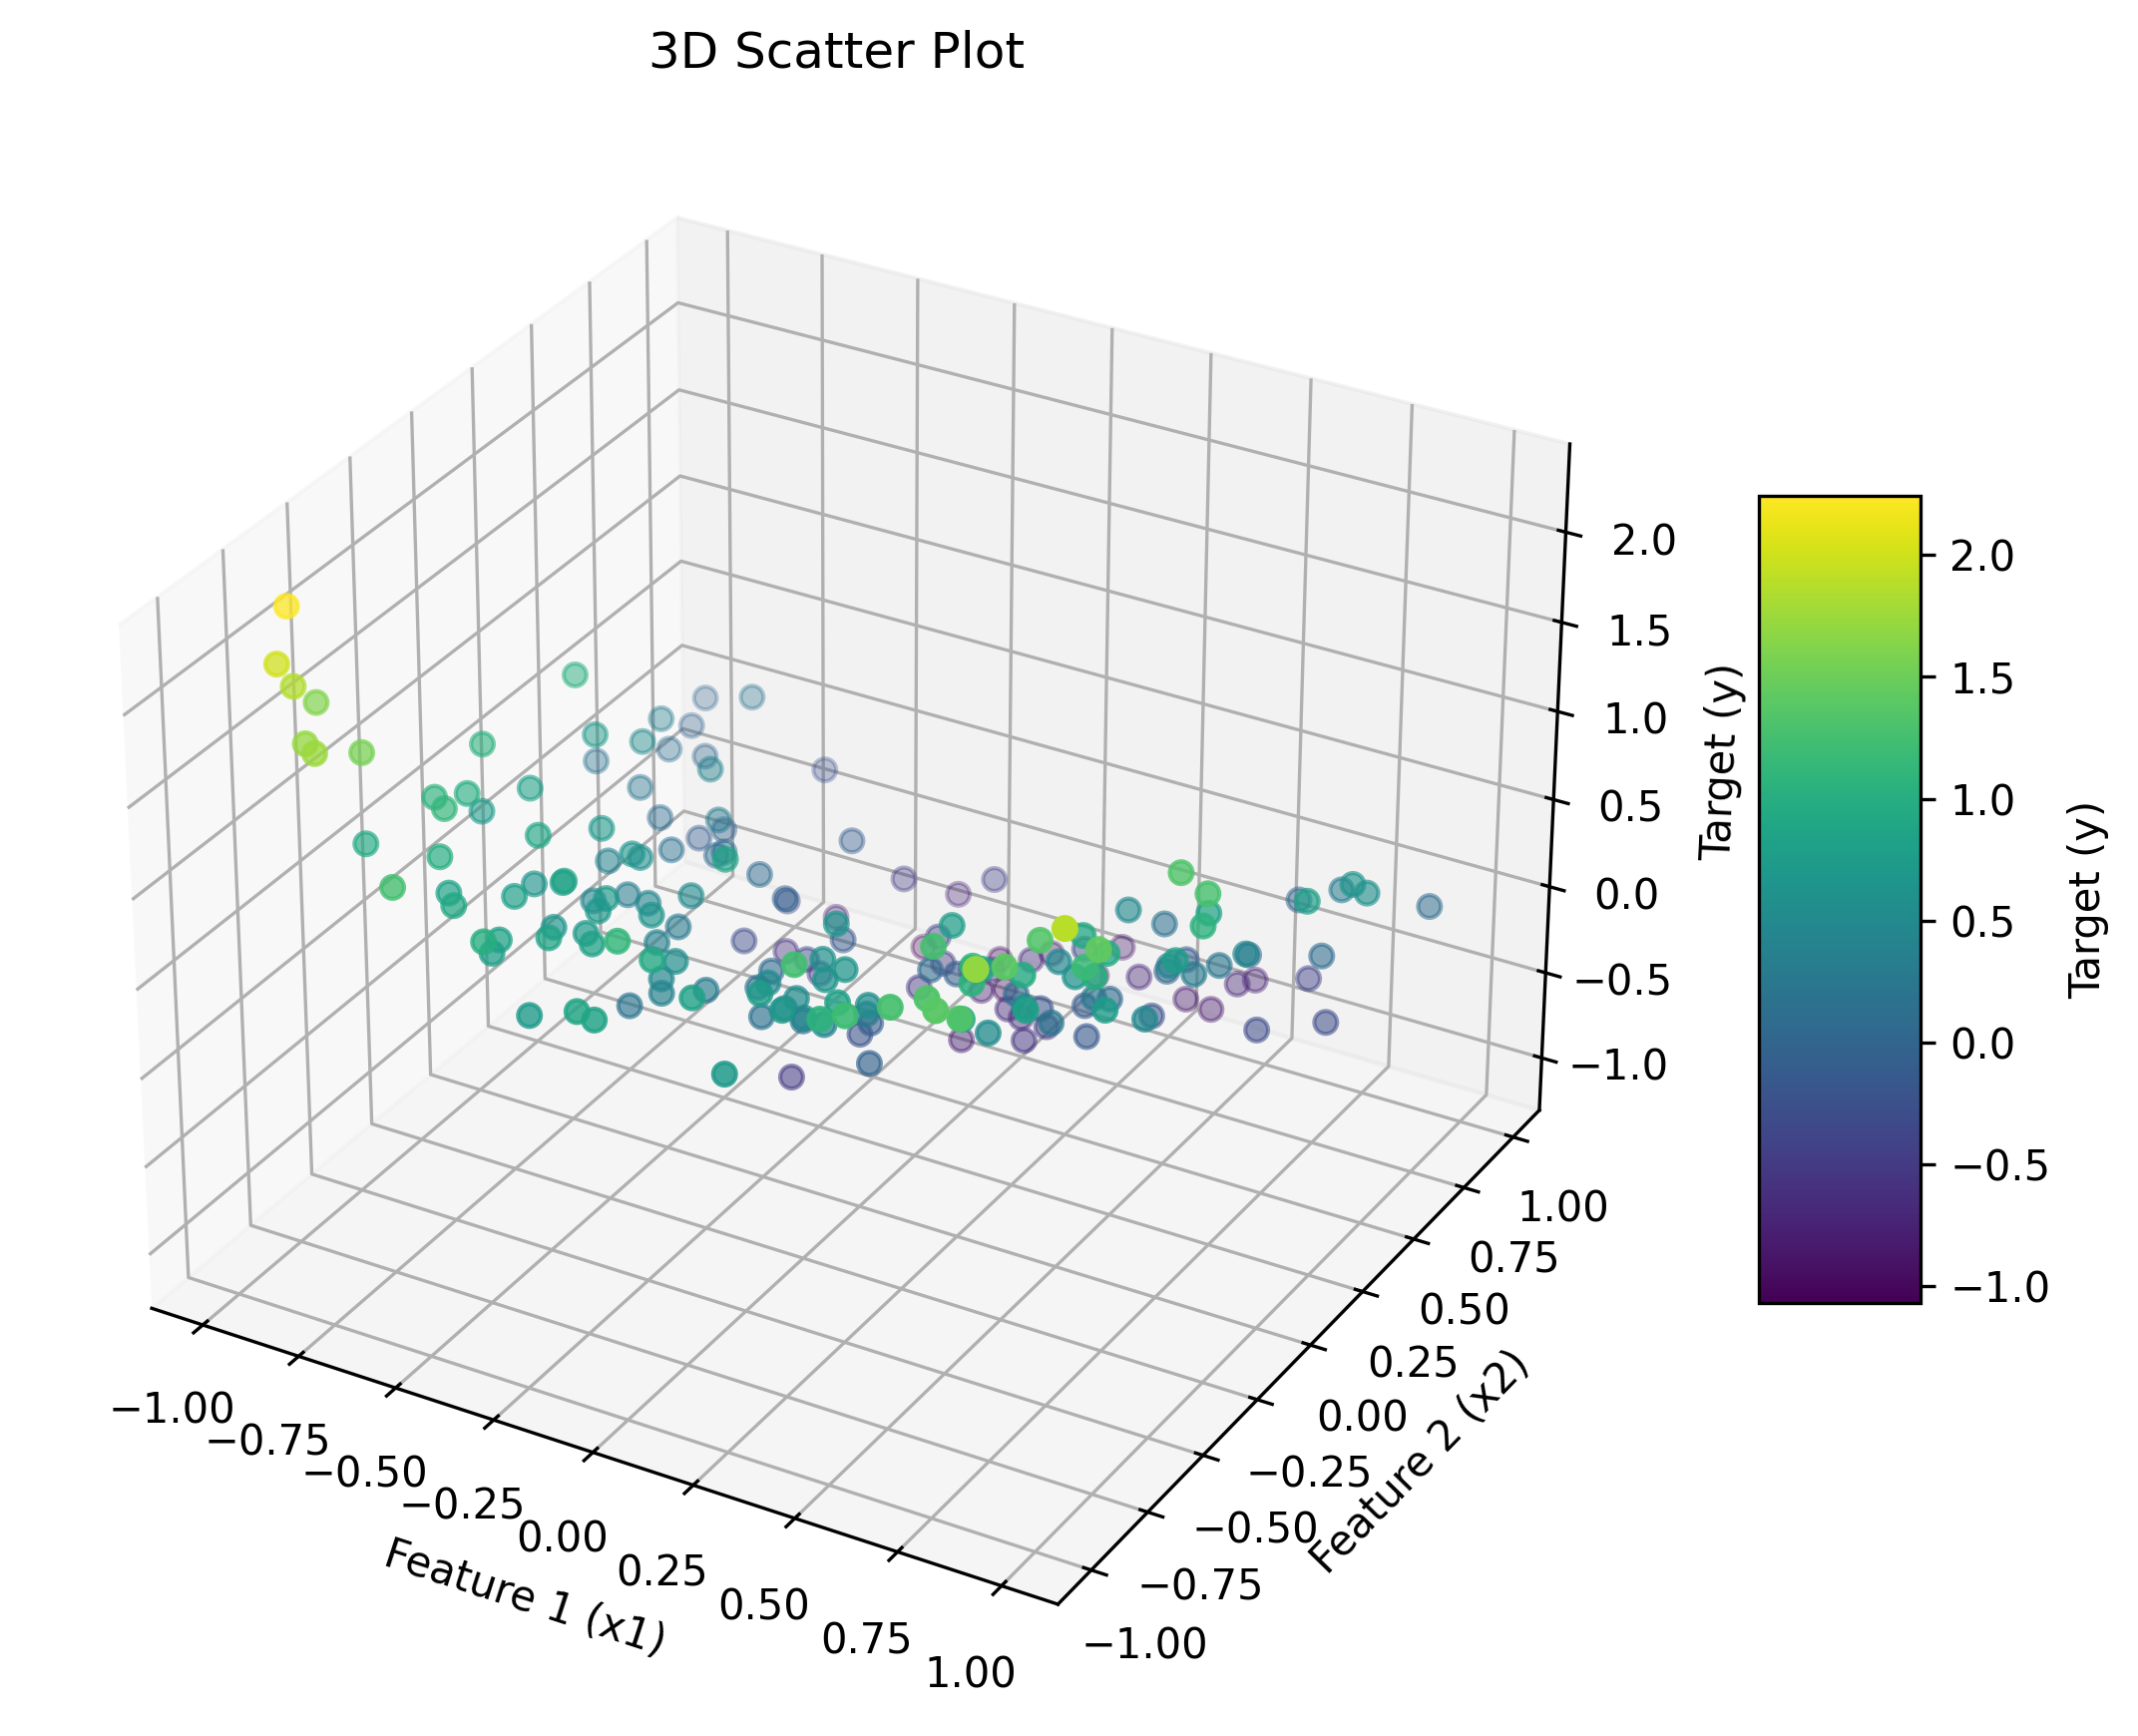
\includegraphics[width=0.7\textwidth]{figures/02_3d_scatter_plot.png}
\caption{3D scatter plot of the data}
\label{fig:3d_scatter}
\end{figure}

Observing the scatter plot, the data seems to look curved and not flat. Also, from the color gradient that the target values follow, it seems like its a non-linear pattern so if I tried fitting just a plane (linear model) to this it wouldn't work well. This tells me I need polynomial features to capture the non-linear patterns.

\subsection*{(i)(b)}

I created polynomial features up to degree 5, which gives 21 features total:

\begin{lstlisting}
from sklearn.preprocessing import PolynomialFeatures
from sklearn.linear_model import Lasso

poly = PolynomialFeatures(degree=5, include_bias=True)
Xpoly = poly.fit_transform(X)
\end{lstlisting}

The 21 features are: 1, $x_1$, $x_2$, $x_1^2$, $x_1x_2$, $x_2^2$, $x_1^3$, $x_1^2x_2$, $x_1x_2^2$, $x_2^3$, $x_1^4$, $x_1^3x_2$, $x_1^2x_2^2$, $x_1x_2^3$, $x_2^4$, $x_1^5$, $x_1^4x_2$, $x_1^3x_2^2$, $x_1^2x_2^3$, $x_1x_2^4$, $x_2^5$

Then I trained Lasso models with different $C$ values. I used $\alpha = 1/(2C)$ through a helper function. I have used MSE as an abbreviation for Mean Squared Error in the document.

\begin{lstlisting}
def C_to_alpha(C):
    return 1.0/(2.0*C)

C_values = [0.001, 0.01, 0.1, 1, 10, 100, 1000]

for C in C_values:
    model = Lasso(alpha=C_to_alpha(C), max_iter=10000)
    model.fit(Xpoly, y)
\end{lstlisting}

\textbf{Results:}

\begin{table}[H]
\centering
\begin{tabular}{ccc}
\toprule
C & Non-zero Coefficients & Training MSE \\
\midrule
0.001 & 0 & 0.4574 \\
0.01 & 0 & 0.4574 \\
0.1 & 0 & 0.4574 \\
1 & 0 & 0.4574 \\
10 & 2 & 0.0772 \\
100 & 2 & 0.0392 \\
1000 & 10 & 0.0368 \\
\bottomrule
\end{tabular}
\end{table}

When $C$ is small (0.001 to 1), the regularization is really strong, infact it was so strong that all coefficients got pushed to zero. The model just predicts a constant value, which gives bad MSE.

At $C=10$, finally two coefficients become non-zero: $x_2$ and $x_1^2$. As $C$ increases further (100, 1000), more coefficients become non-zero and the training error goes down.

\textbf{Detailed coefficients for all C values:}

\begin{table}[H]
\centering
\small
\begin{tabular}{lccccccc}
\toprule
Feature & C=0.001 & C=0.01 & C=0.1 & C=1 & C=10 & C=100 & C=1000 \\
\midrule
$x_2$ & 0 & 0 & 0 & 0 & -0.845 & -0.988 & -1.049 \\
$x_1^2$ & 0 & 0 & 0 & 0 & 0.510 & 1.060 & 1.109 \\
$x_1x_2$ & 0 & 0 & 0 & 0 & 0 & 0 & -0.180 \\
$x_1^3$ & 0 & 0 & 0 & 0 & 0 & 0 & -0.012 \\
$x_1^2x_2$ & 0 & 0 & 0 & 0 & 0 & 0 & 0.045 \\
$x_1^3x_2$ & 0 & 0 & 0 & 0 & 0 & 0 & 0.213 \\
$x_1^4x_2$ & 0 & 0 & 0 & 0 & 0 & 0 & -0.094 \\
$x_1^3x_2^2$ & 0 & 0 & 0 & 0 & 0 & 0 & -0.008 \\
$x_1x_2^4$ & 0 & 0 & 0 & 0 & 0 & 0 & -0.033 \\
$x_2^5$ & 0 & 0 & 0 & 0 & 0 & 0 & 0.125 \\
\bottomrule
\end{tabular}
\end{table}

\subsection*{(i)(c)}

My data goes from about -1 to 1, so I extended the grid to about -3 to 3, I generated it on a grid to extend it beyond the training data range:

\begin{lstlisting}
x1_range = X[:,0].max() - X[:,0].min()
x2_range = X[:,1].max() - X[:,1].min()
x1_min = X[:,0].min() - 1.0*x1_range
x1_max = X[:,0].max() + 1.0*x1_range
x2_min = X[:,1].min() - 1.0*x2_range
x2_max = X[:,1].max() + 1.0*x2_range

x1_grid = np.linspace(x1_min, x1_max, 60)
x2_grid = np.linspace(x2_min, x2_max, 60)
X1_mesh, X2_mesh = np.meshgrid(x1_grid, x2_grid)

Xg = np.c_[X1_mesh.ravel(), X2_mesh.ravel()]
Xg_poly = poly.transform(Xg)
Z = model.predict(Xg_poly).reshape(X1_mesh.shape)

fig = plt.figure()
ax = fig.add_subplot(111, projection='3d')
ax.plot_surface(X1_mesh, X2_mesh, Z, alpha=0.6, cmap='viridis')
ax.scatter(X[:,0], X[:,1], y, c='red', s=30)
plt.show()
\end{lstlisting}

I plotted surfaces for $C = 0.001$, $C = 1$, and $C = 1000$.

\begin{itemize}
    \item \textbf{C = 0.001}: Almost completely flat surface. The model is totally underfitting, it seems to just predict roughly the mean value everywhere because all coefficients are zero.
    
    \item \textbf{C = 1}: Still flat. Same problem, the regularization is too strong.
    
    \item \textbf{C = 1000}: Now we see a curved surface that fits the data points pretty well. The model captures the patterns well but maybe its starting to overfit at this point.
\end{itemize}

As $C$ increases, the prediction surface goes from flat (underfitting) to curved (better fit), we can see this in the image below.

\begin{figure}[H]
\centering
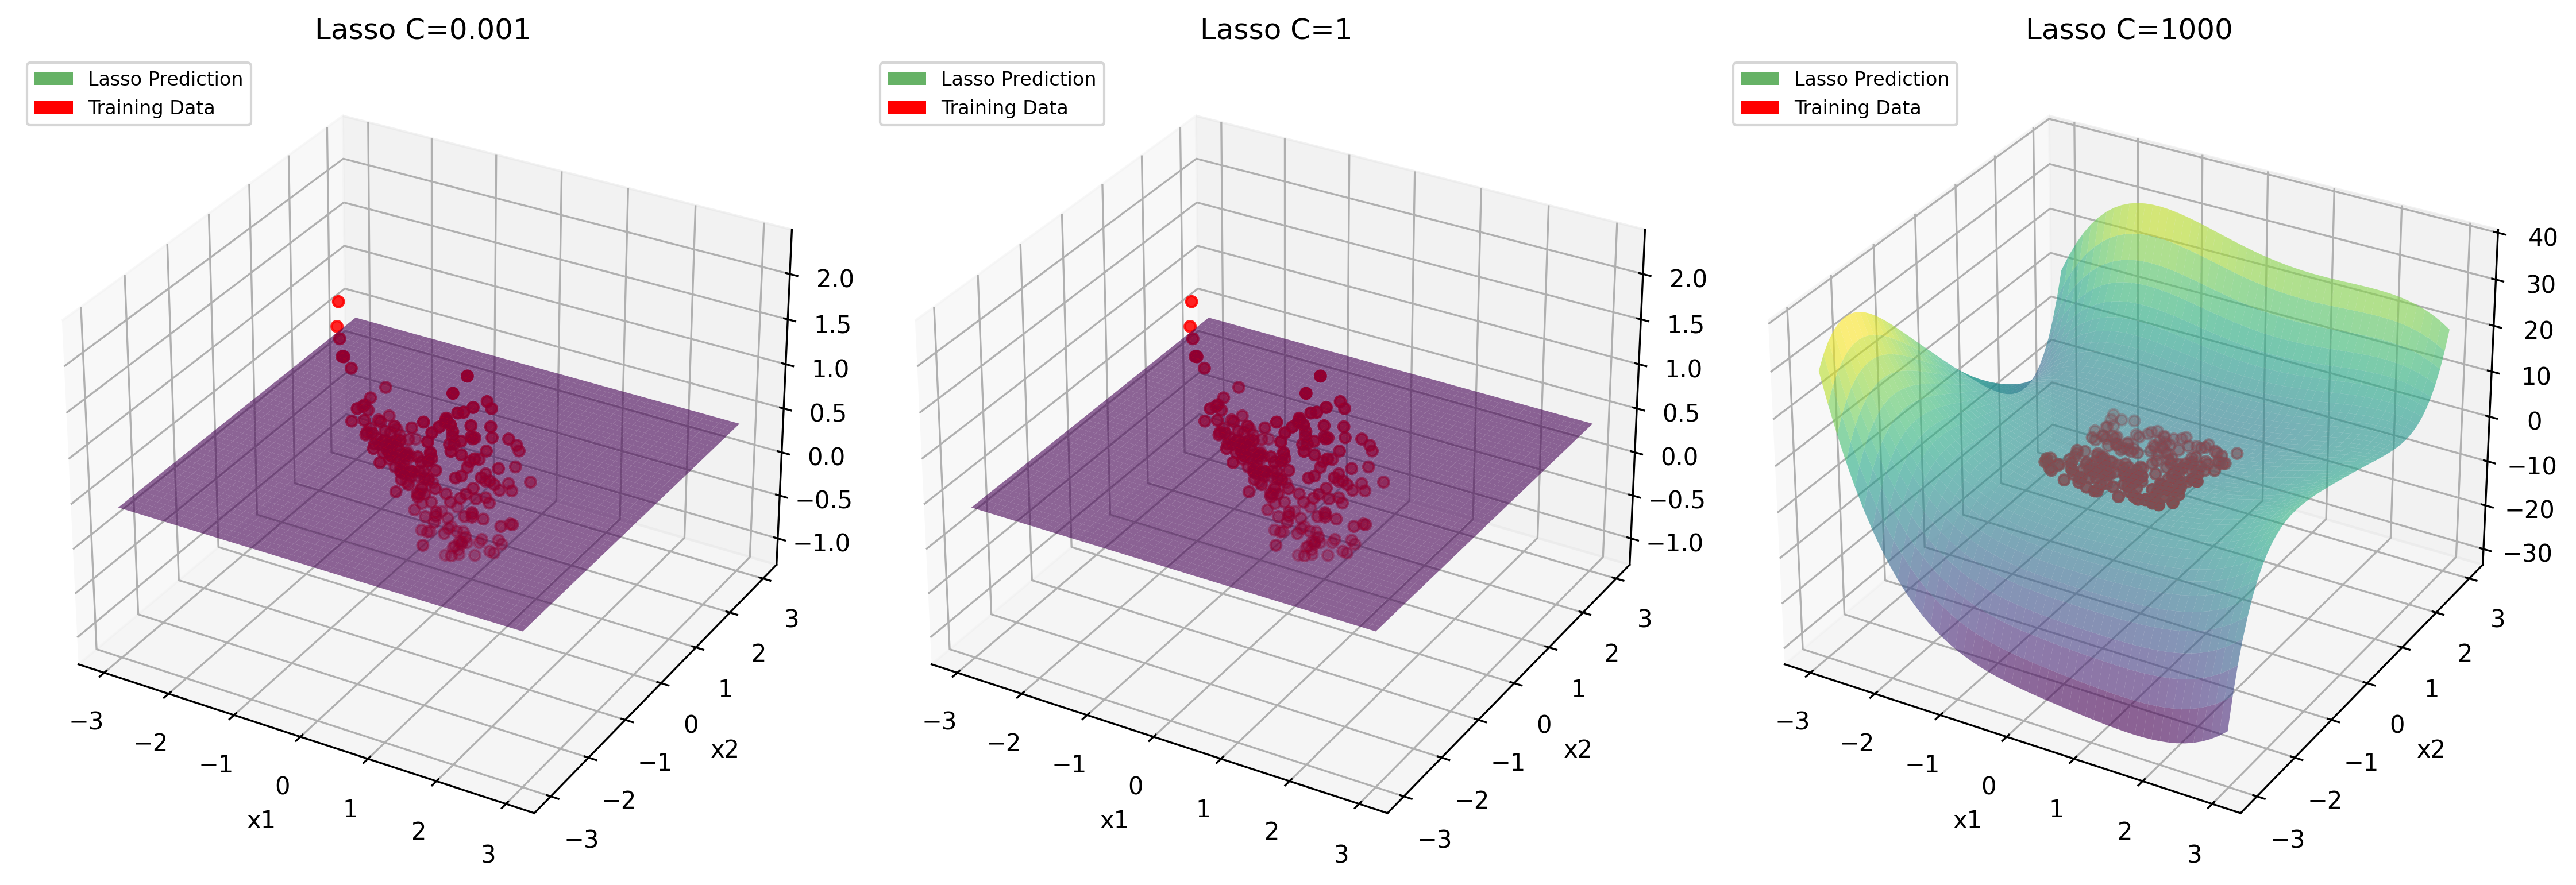
\includegraphics[width=0.95\textwidth]{figures/03_lasso_prediction_surfaces.png}
\caption{Lasso prediction surfaces for different C values (0.001, 1, 1000). The surfaces (colored) show model predictions on an extended grid, and red points show the training data.}
\label{fig:lasso_surfaces}
\end{figure}

\subsection*{(i)(d)}

Underfitting is when the model is too simple to learn any real patterns from the data. This occurs in Lasso when $C$ is too small and the regularization is too strong. The bias here is high (the model is biased to be too simple) and the variance is low (predictions won't change much with different training sets), and both the training and test error are high.

Overfitting is when the model is too complex and starts to fit the noise in the training data, again indicating a pattern in the actual training data. Here, the bias is low but the variance is high (predictions change a lot with different training data), and this is the situation you encounter when $C$ is too large, then the training error is low and the test error is high.

\textbf{How C controls this trade-off:}

The $C$ parameter controls the strength of regularization through the penalty term:

\begin{equation}
J(\theta) = \frac{1}{m} \sum_{i=1}^{m} (h_\theta(x^{(i)}) - y^{(i)})^2 + \frac{1}{C} \sum_{j=1}^{n} |\theta_j|
\end{equation}

\begin{itemize}
    \item When C is small, the strong regularization penalty forces most coefficients to zero, creating an overly simple model that underfits.
    \item When C is large, the weak regularization allows many non-zero coefficients, creating a complex model that potentially risks overfitting.
\end{itemize}

From my results:
\begin{itemize}
    \item $C \leq 1$: Definitely underfitting (0 non-zero coefficients, MSE = 0.4574)
    \item $C = 10$: Starting to fit (2 coefficients, MSE = 0.0772)
    \item $C = 100$: Good fit (2 coefficients, MSE = 0.0392)
    \item $C = 1000$: Possibly overfitting (10 coefficients, MSE = 0.0368)
\end{itemize}

The sweet spot is somewhere around $C = 10$-$100$ where we balance complexity and regularization.

\begin{figure}[H]
\centering
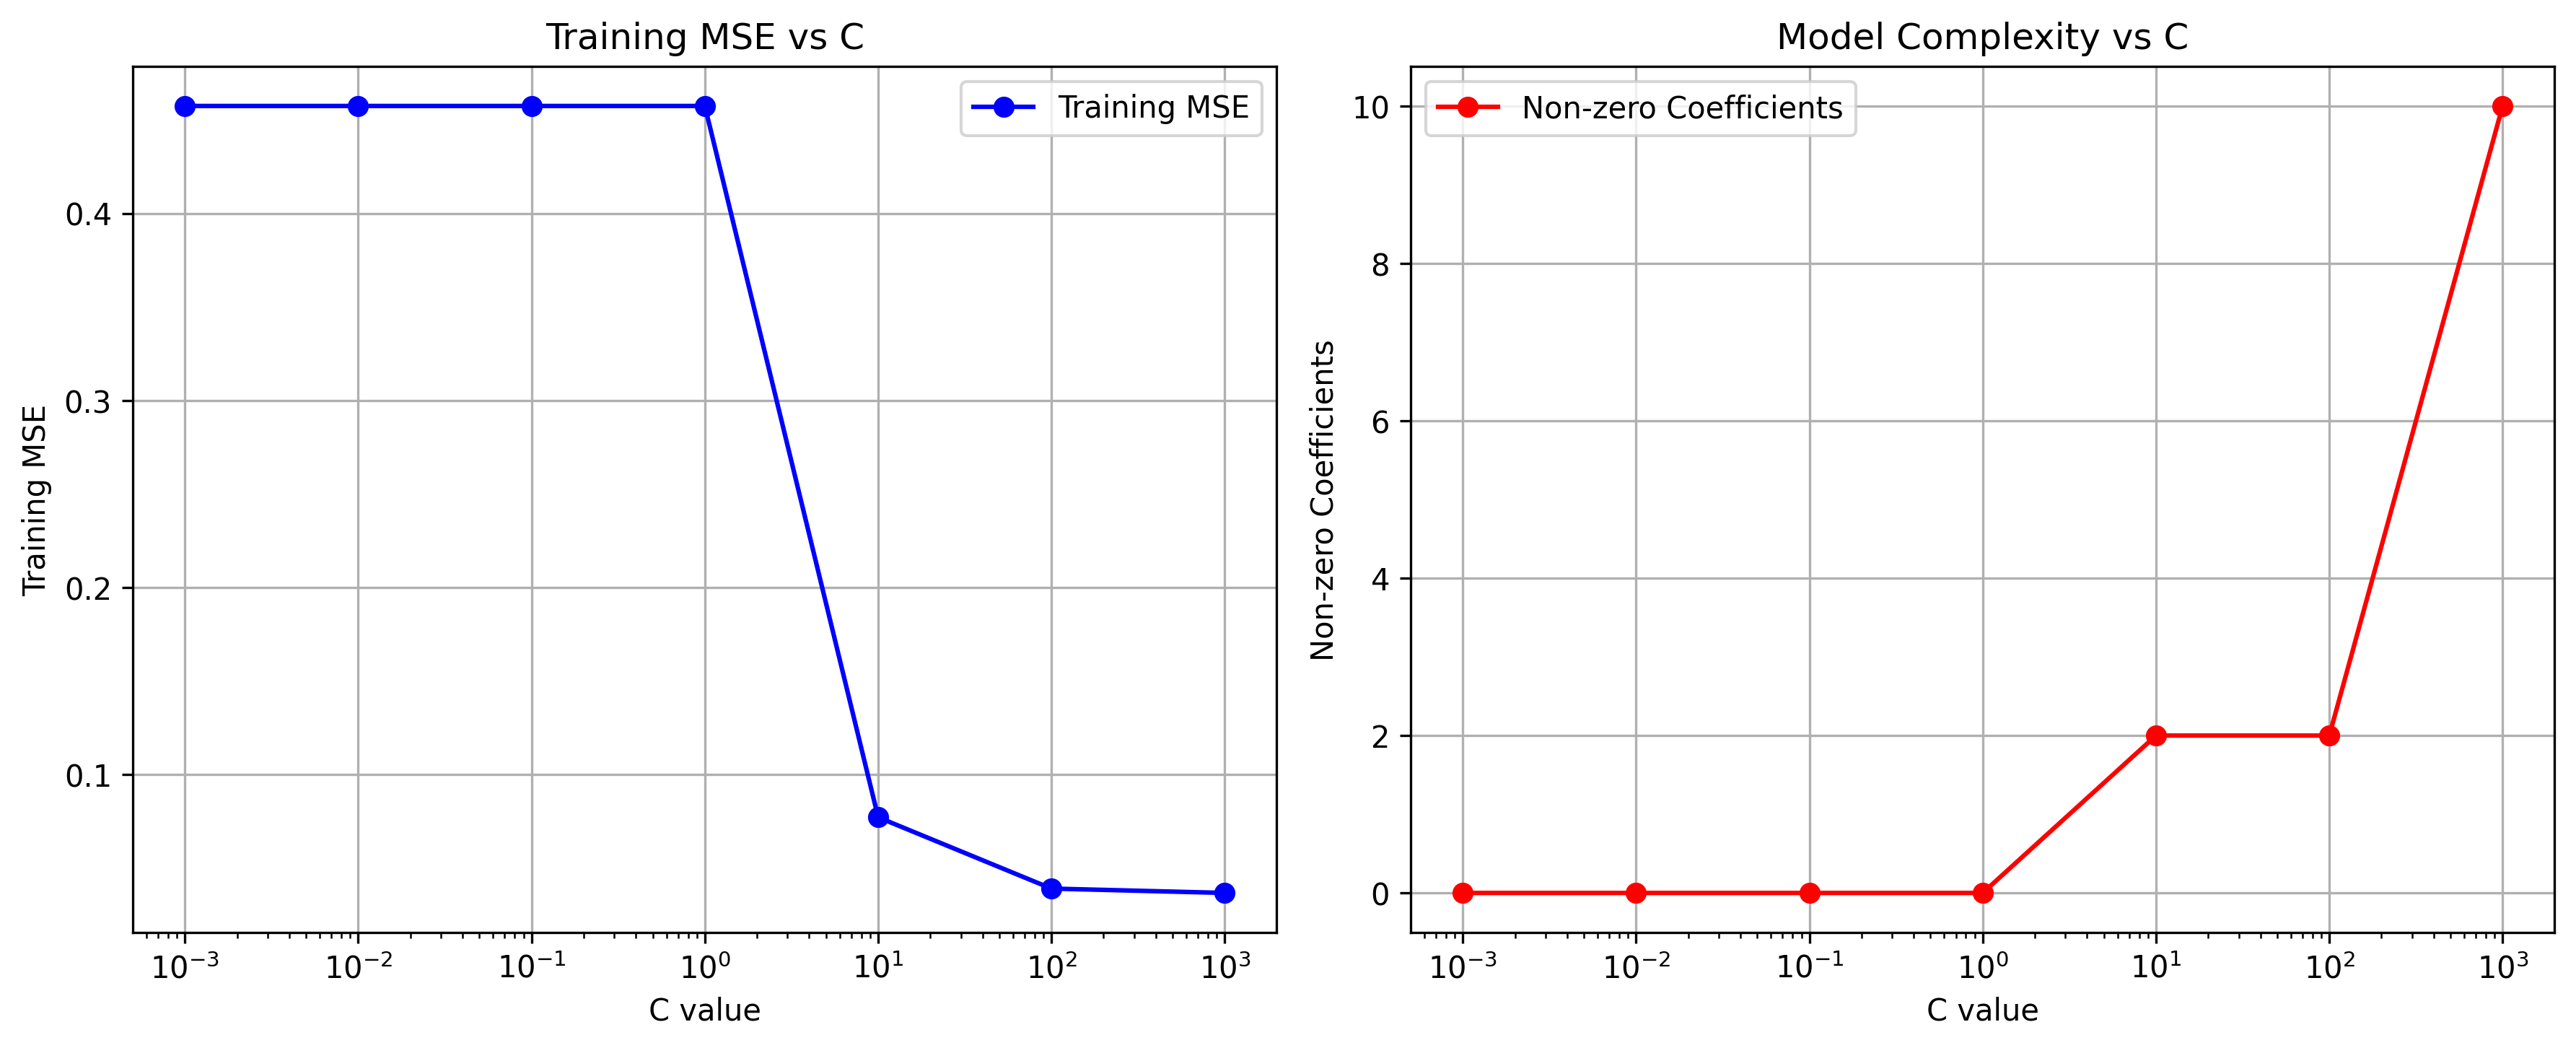
\includegraphics[width=0.95\textwidth]{figures/04_underfitting_overfitting_analysis.png}
\caption{Left: Training MSE decreases as C increases (less regularization). Right: Number of non-zero coefficients increases with C, showing the model becoming more complex.}
\label{fig:underfitting_overfitting}
\end{figure}

\subsection*{(i)(e)}

Ridge regression uses $L_2$ penalty instead of $L_1$:

\begin{equation}
J(\theta) = \frac{1}{m} \sum_{i=1}^{m} (h_\theta(x^{(i)}) - y^{(i)})^2 + \frac{1}{C} \theta^T\theta
\end{equation}

\begin{lstlisting}
from sklearn.linear_model import Ridge

for C in C_values:
    model = Ridge(alpha=C_to_alpha(C))
    model.fit(Xpoly, y)
\end{lstlisting}

\textbf{Ridge Results:}

\begin{table}[H]
\centering
\begin{tabular}{cc}
\toprule
C & Training MSE \\
\midrule
0.001 & 0.3467 \\
0.01 & 0.1211 \\
0.1 & 0.0455 \\
1 & 0.0370 \\
10 & 0.0351 \\
100 & 0.0349 \\
1000 & 0.0349 \\
\bottomrule
\end{tabular}
\end{table}

Lasso sets coefficients to \textit{exactly} zero ($L_1$ penalty), while Ridge just makes them small ($L_2$ penalty). We can see this at $C=1$:

\begin{table}[H]
\centering
\small
\begin{tabular}{lcc|lcc}
\toprule
Feature & Lasso & Ridge & Feature & Lasso & Ridge \\
\midrule
1 & 0.000 & -0.809 & $x_1^3x_2$ & 0.000 & 0.183 \\
$x_1$ & 0.000 & -0.003 & $x_1^2x_2^2$ & 0.000 & 0.034 \\
$x_2$ & 0.000 & -1.019 & $x_1x_2^3$ & 0.000 & 0.055 \\
$x_1^2$ & 0.000 & 0.909 & $x_2^4$ & 0.000 & 0.034 \\
$x_1x_2$ & 0.000 & -0.199 & $x_1^5$ & 0.000 & 0.087 \\
$x_2^2$ & 0.000 & -0.051 & $x_1^4x_2$ & 0.000 & -0.149 \\
$x_1^3$ & 0.000 & -0.076 & $x_1^3x_2^2$ & 0.000 & -0.103 \\
$x_1^2x_2$ & 0.000 & 0.088 & $x_1^2x_2^3$ & 0.000 & -0.037 \\
$x_1x_2^2$ & 0.000 & 0.118 & $x_1x_2^4$ & 0.000 & -0.112 \\
$x_2^3$ & 0.000 & -0.062 & $x_2^5$ & 0.000 & 0.154 \\
$x_1^4$ & 0.000 & 0.198 & & & \\
\bottomrule
\end{tabular}
\caption*{Coefficient comparison at C=1: Lasso has all zeros (strong regularization), while Ridge has small non-zero values for all 21 features.}
\end{table}

When changing the C parameter, Lasso and Ridge regression show fundamentally different behaviors in their model parameters. As C increases in Lasso, coefficients transition from exactly zero to non-zero values in an abrupt, discontinuous manner due to the $L_1$ penalty, for example, at $C=1$ all 21 coefficients are zero, but at $C=10$ suddenly 2 coefficients become active. In contrast, Ridge regression with $L_2$ penalty makes smooth, gradual changes in all coefficients as C increases; all 21 coefficients retain non-zero values at every value of C, just increasing continuously from very small values (highly shrunk at low C) to larger values (less shrunk at high C). Thus, Lasso does automatic feature selection by dropping irrelevant features entirely and is ideal when we believe only a few features are truly predictive while Ridge maintains all features with varying degrees of shrinkage and is preferable when we believe that most features contribute something to the prediction. Finally, given that Ridge uses all the features rather than dropping some irrelevant ones entirely, Ridge generally has lower training MSE than Lasso with the same value of C.

\begin{figure}[H]
\centering
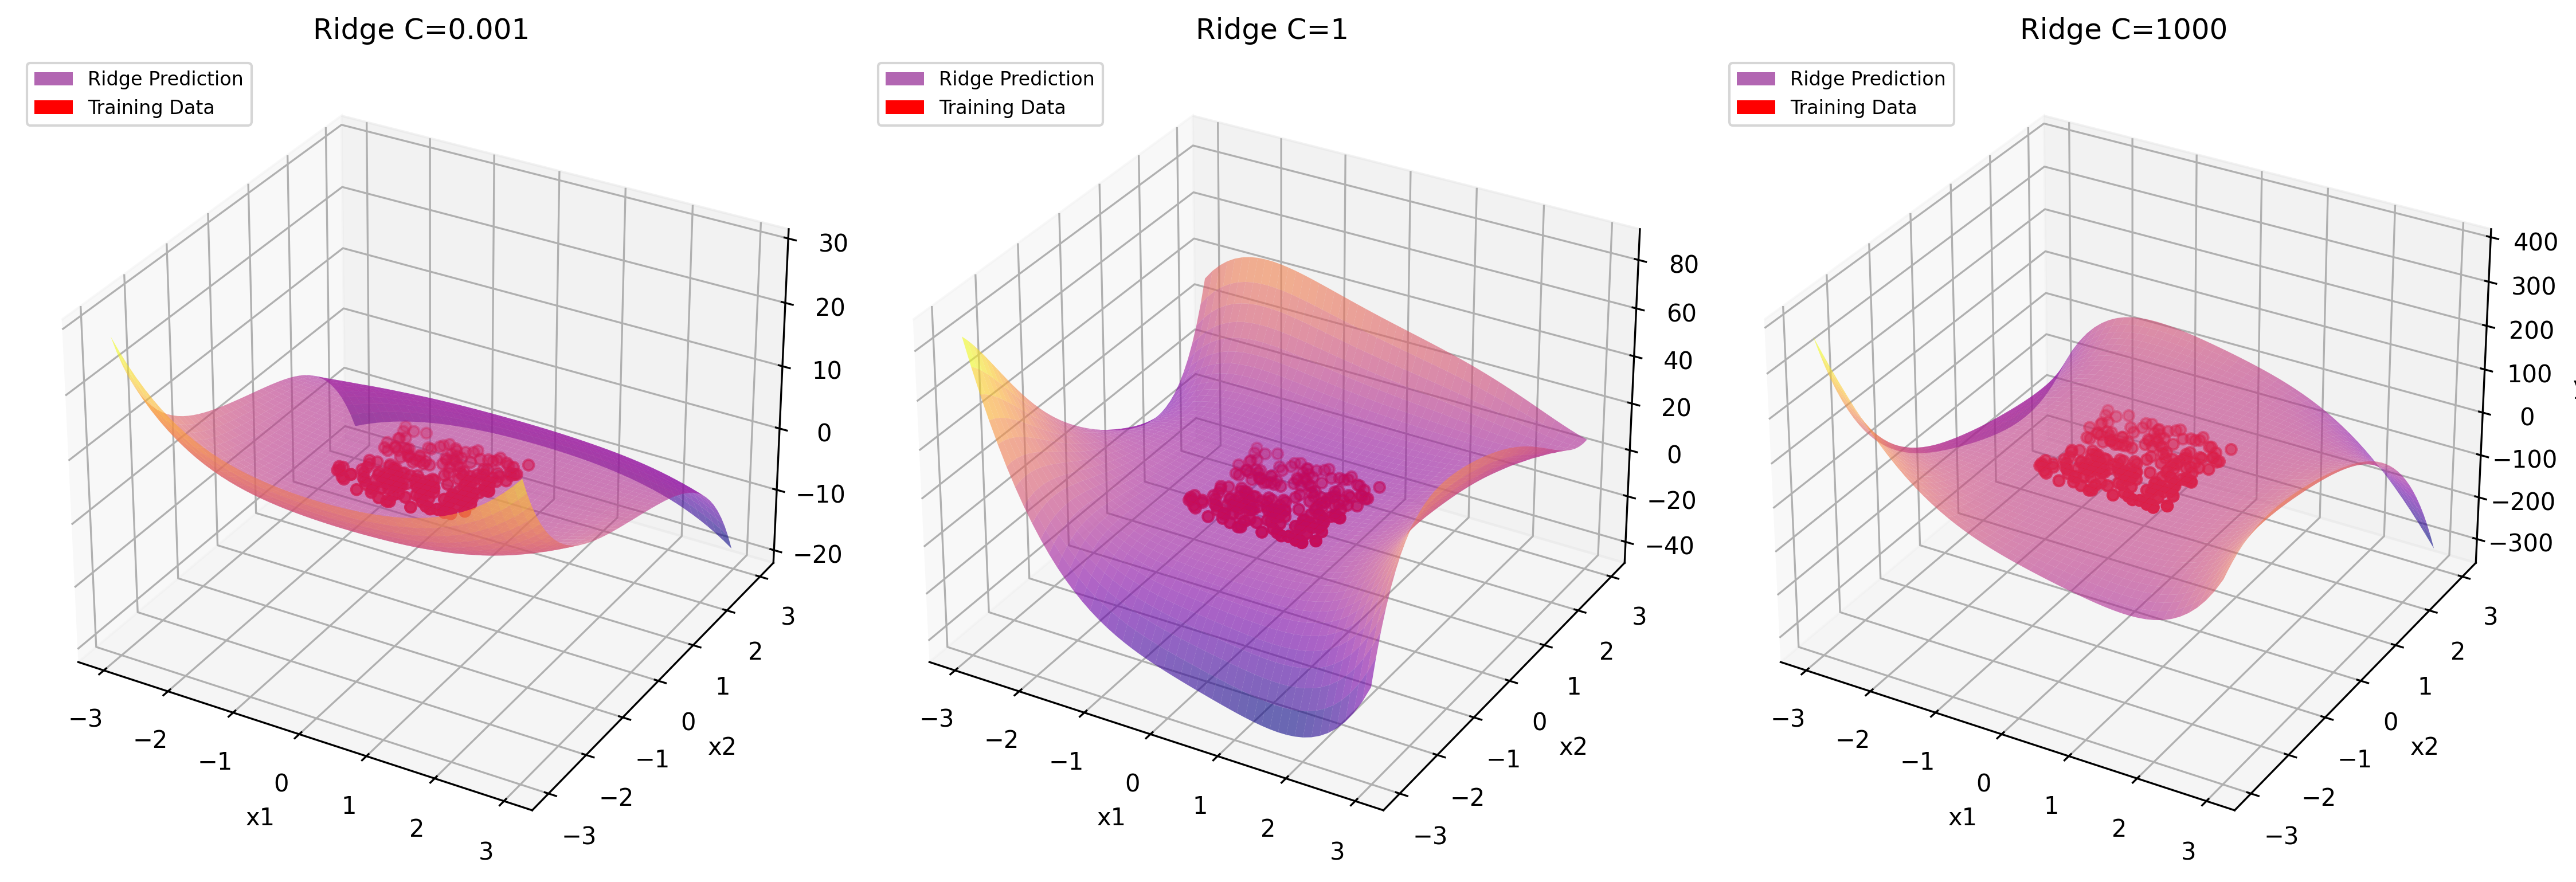
\includegraphics[width=0.95\textwidth]{figures/05_ridge_prediction_surfaces.png}
\caption{Ridge prediction surfaces for different C values (0.001, 1, 1000). Unlike Lasso, Ridge produces smooth transitions between regularization levels without setting coefficients to exactly zero.}
\label{fig:ridge_surfaces}
\end{figure}

\subsection*{(ii)(a)}

I used 5-fold cross validation to find the best $C$ value. Split the data into 5 parts, train on 4 parts and test on the 5th, repeat for all combinations:

\begin{lstlisting}
from sklearn.model_selection import KFold

kf = KFold(n_splits=5, shuffle=True, random_state=42)
C_cv = [0.001, 0.01, 0.1, 0.5, 1, 2, 5, 10, 50, 100, 500, 1000]

cv_means = []
cv_stds = []

for C in C_cv:
    scores = []
    for train_idx, val_idx in kf.split(Xpoly):
        model = Lasso(alpha=C_to_alpha(C), max_iter=10000)
        model.fit(Xpoly[train_idx], y[train_idx])
        pred = model.predict(Xpoly[val_idx])
        scores.append(mean_squared_error(y[val_idx], pred))
    
    cv_means.append(np.mean(scores))
    cv_stds.append(np.std(scores))

plt.errorbar(C_cv, cv_means, yerr=cv_stds, fmt='o-', capsize=5)
plt.xscale('log')
plt.xlabel('C value')
plt.ylabel('CV MSE')
plt.show()
\end{lstlisting}

I started small (0.001) where regularization is super strong, and went up to 1000 where it's very weak. Used 12 different values to get a good picture of what's happening. It is suggested we increase by factors of 5 or 10, which is roughly what I did.

\textbf{Cross Validation Results:}

\begin{table}[H]
\centering
\begin{tabular}{ccc}
\toprule
C & Mean Cross Validation MSE & Standard Deviation \\
\midrule
0.001 & 0.4670 & 0.1241 \\
0.01 & 0.4670 & 0.1241 \\
0.1 & 0.4670 & 0.1241 \\
0.5 & 0.4670 & 0.1241 \\
1 & 0.4670 & 0.1241 \\
2 & 0.3571 & 0.1239 \\
5 & 0.1801 & 0.0552 \\
10 & 0.0814 & 0.0260 \\
50 & 0.0416 & 0.0119 \\
\textbf{100} & \textbf{0.0408} & \textbf{0.0119} \\
500 & 0.0419 & 0.0135 \\
1000 & 0.0429 & 0.0146 \\
\bottomrule
\end{tabular}
\end{table}

The error bars represent the standard deviation across the 5 folds. Allows us to pull information about the reliability of the model, with a small standard deviation indicating the model is consistent across the train/test splits, versus a large standard deviation indicating that the models performance varies substantially with the data it sees. This in turn allows the selection of a model that we deem not just the lowest mean error, but also reliable.

\begin{figure}[H]
\centering
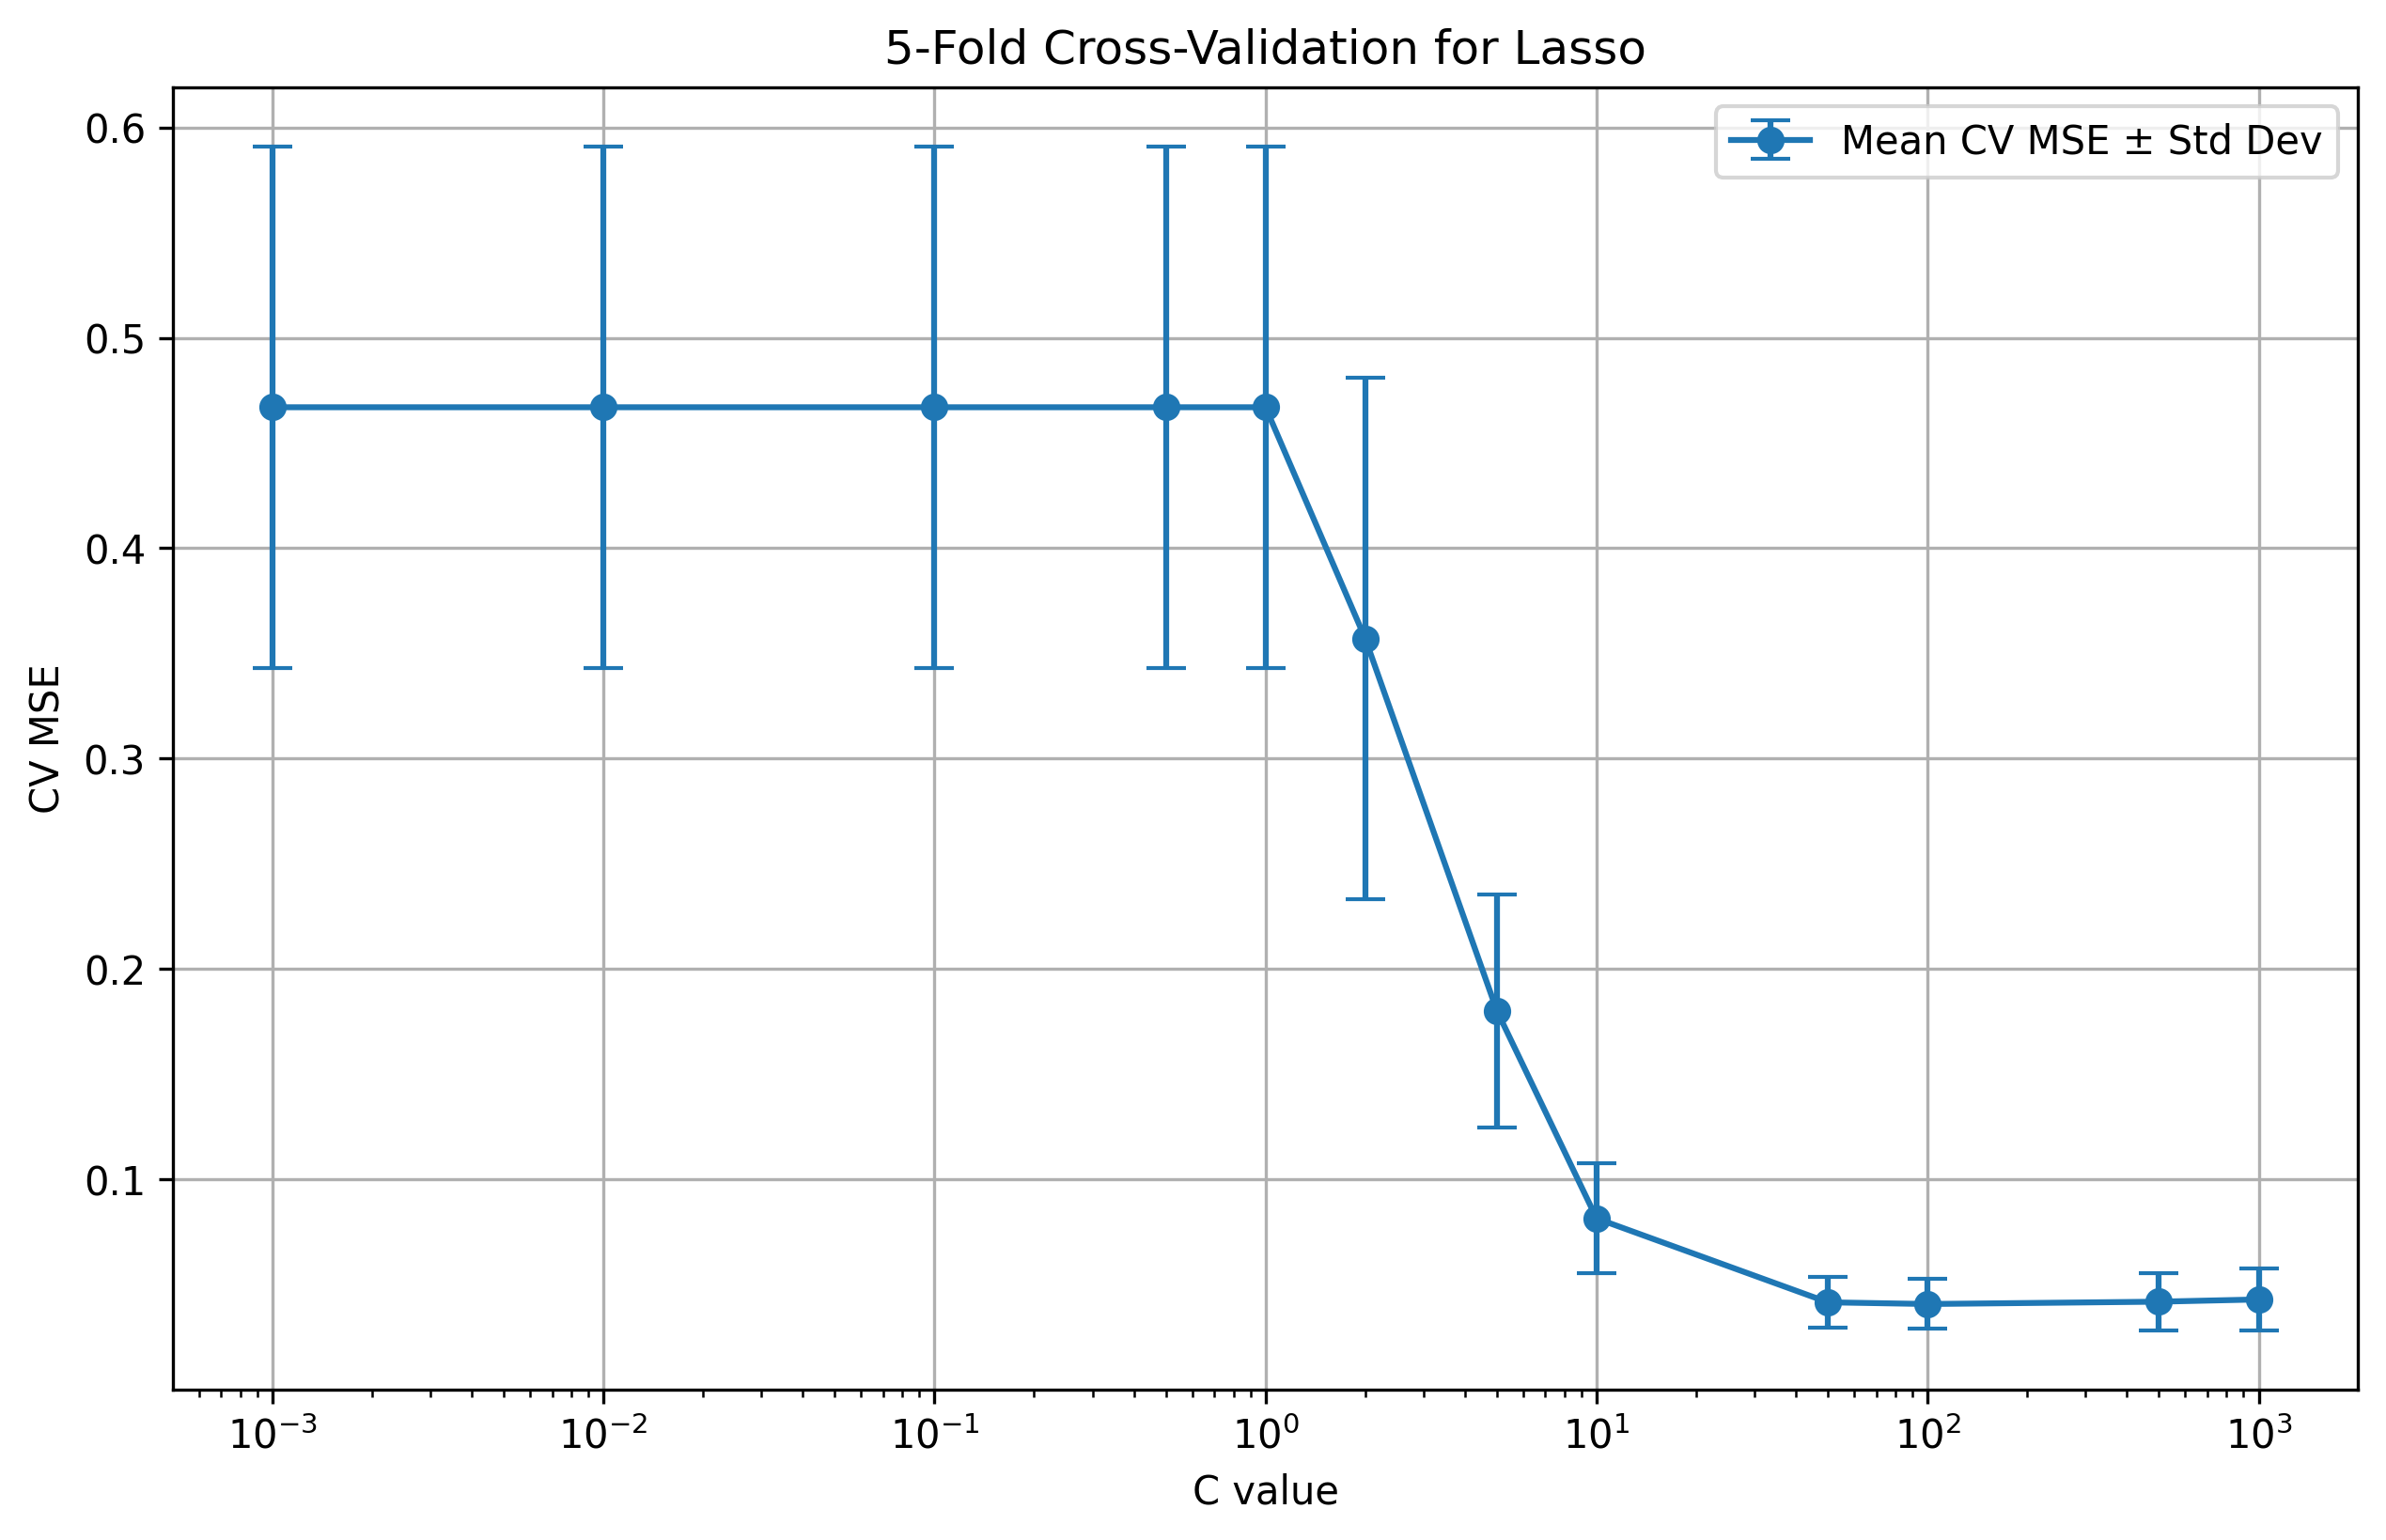
\includegraphics[width=0.8\textwidth]{figures/06_lasso_cv_results.png}
\caption{5-fold cross-validation results for Lasso. The error bars represent standard deviation across folds. The optimal C value is 100, where CV MSE is minimized.}
\label{fig:lasso_cv}
\end{figure}

\subsection*{(ii)(b)}

I would choose C = 100 because it achieves the lowest cross-validation Mean Squared Error of 0.0408 with a reasonable standard deviation of 0.0119, demonstrating stable performance. When C is incremented beyond this value, the error begins to increase, suggesting a concern for overfitting. This optimal Lasso model performs automatic feature selection, retaining only 2 out of 21 polynomial features: $x_2$ with coefficient -0.987955 and $x_1^2$ with coefficient 1.060313, resulting in a sparse, interpretable model with Cross Validation MSE = $0.0408 \pm 0.0119$.

\subsection*{(ii)(c)}

I followed the same procedure for Ridge Regression:

\begin{lstlisting}
ridge_cv_means = []
ridge_cv_stds = []

for C in C_cv:
    scores = []
    for train_idx, val_idx in kf.split(Xpoly):
        model = Ridge(alpha=C_to_alpha(C))
        model.fit(Xpoly[train_idx], y[train_idx])
        pred = model.predict(Xpoly[val_idx])
        scores.append(mean_squared_error(y[val_idx], pred))
    
    ridge_cv_means.append(np.mean(scores))
    ridge_cv_stds.append(np.std(scores))
\end{lstlisting}

\textbf{Ridge Cross Validation Results:}

\begin{table}[H]
\centering
\begin{tabular}{ccc}
\toprule
C & Mean Cross Validation MSE & Standard Deviation \\
\midrule
0.001 & 0.3752 & 0.1071 \\
0.01 & 0.1476 & 0.0476 \\
0.1 & 0.0521 & 0.0164 \\
0.5 & 0.0440 & 0.0140 \\
1 & 0.0435 & 0.0142 \\
2 & 0.0433 & 0.0146 \\
5 & 0.0432 & 0.0151 \\
\textbf{10} & \textbf{0.0431} & \textbf{0.0154} \\
50 & 0.0435 & 0.0161 \\
100 & 0.0437 & 0.0164 \\
500 & 0.0439 & 0.0167 \\
1000 & 0.0440 & 0.0167 \\
\bottomrule
\end{tabular}
\end{table}

For Ridge Regression, I would choose C = 10. The Cross Validation error decreases smoothly as $C$ increases, then levels off around $C=10$ and remains roughly constant. No abrupt jumps like we saw with Lasso Regression.

\begin{figure}[H]
\centering
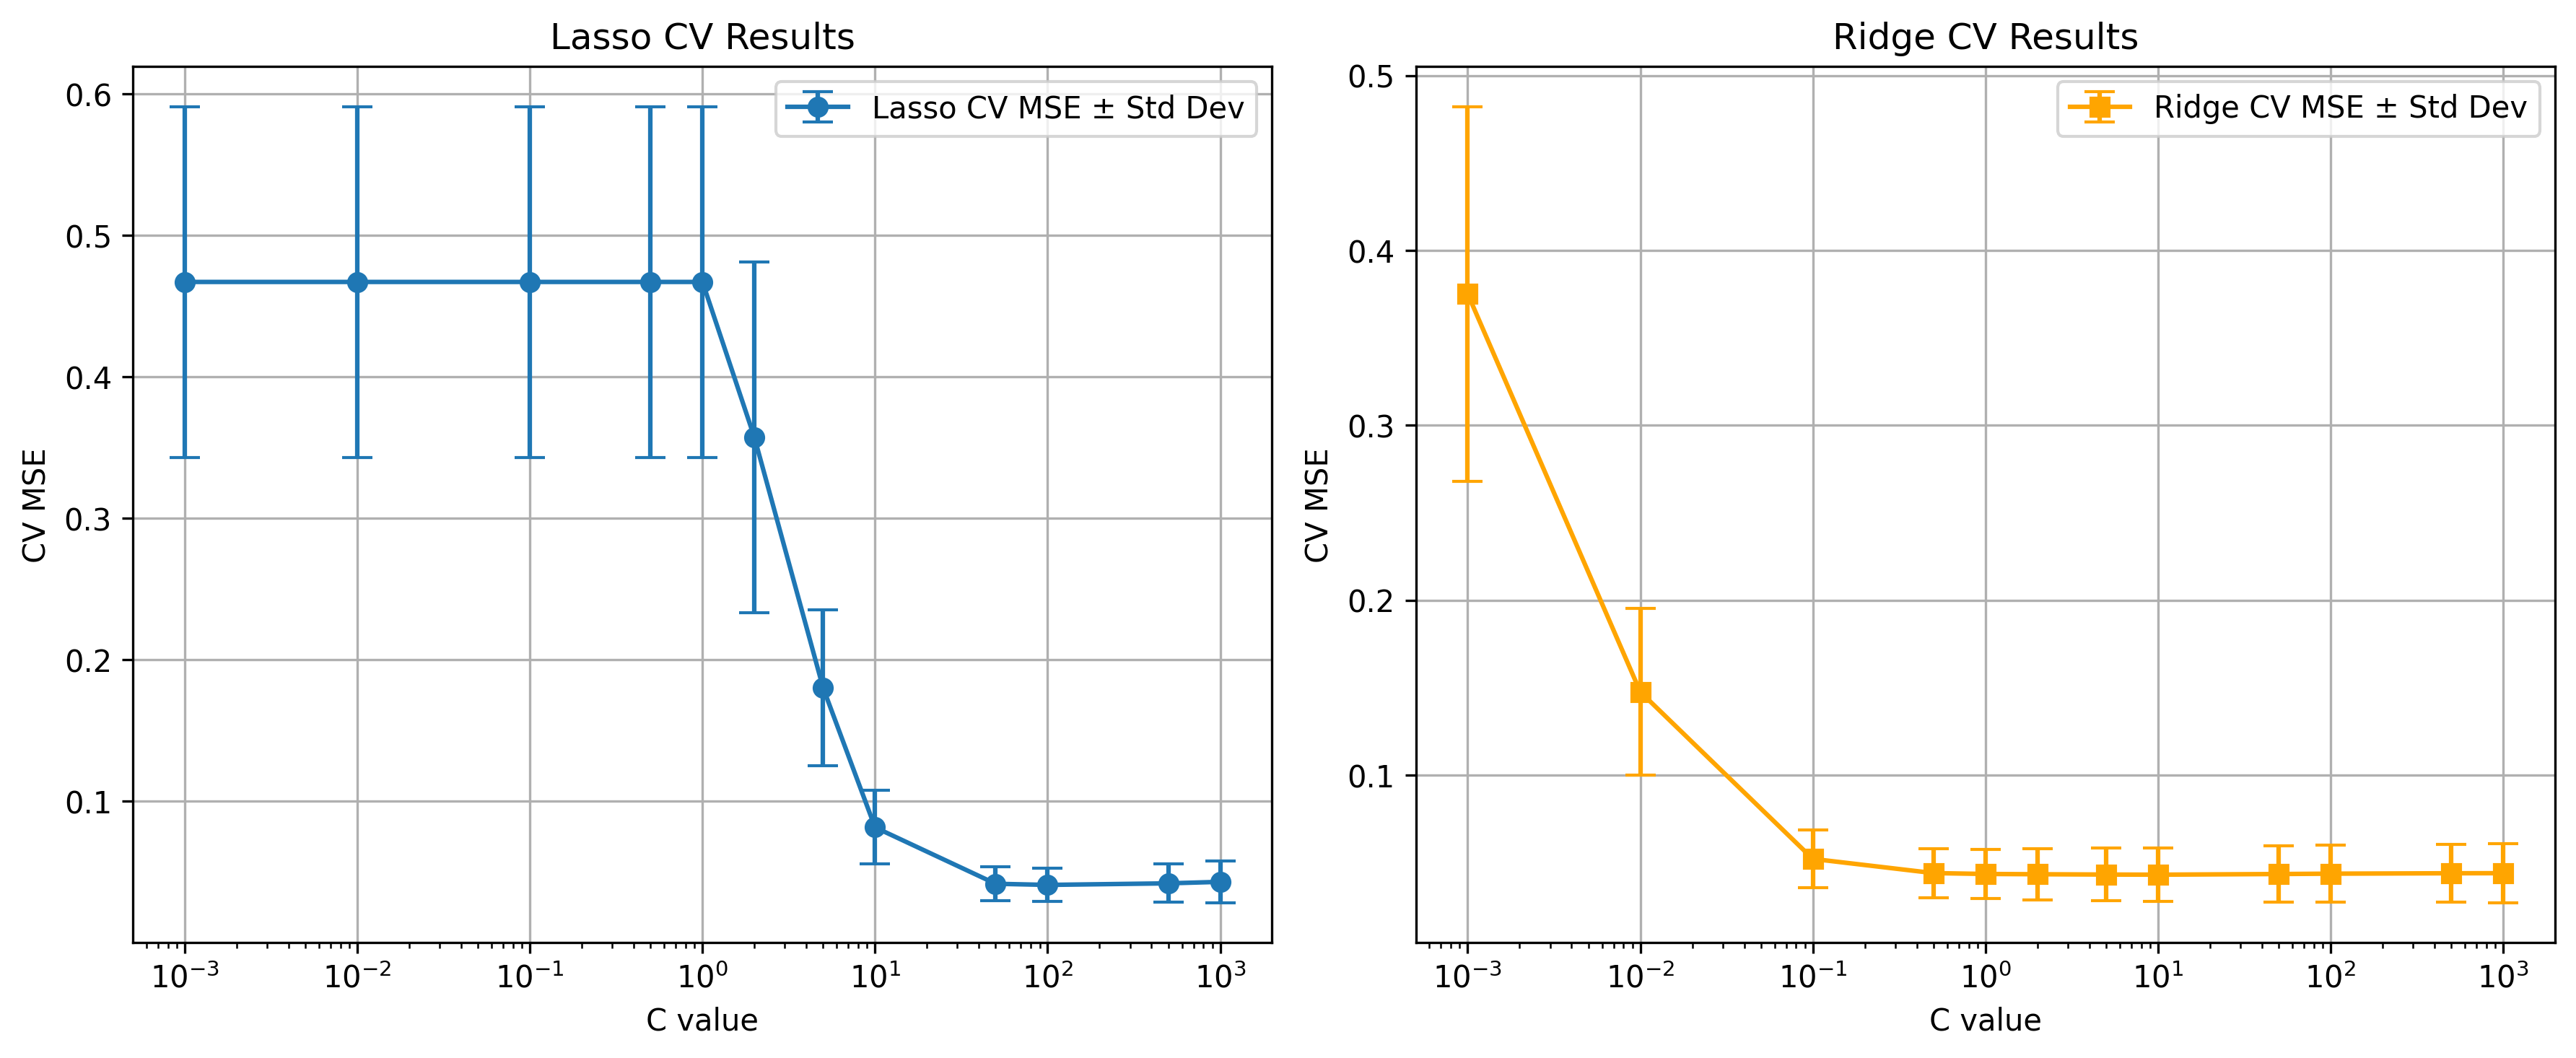
\includegraphics[width=0.95\textwidth]{figures/07_lasso_ridge_cv_comparison.png}
\caption{Side-by-side comparison of 5-fold CV results for Lasso (left) and Ridge (right). Lasso shows a sharp transition around C=2-10, while Ridge shows a smooth gradual improvement.}
\label{fig:cv_comparison}
\end{figure}

\begin{figure}[H]
\centering
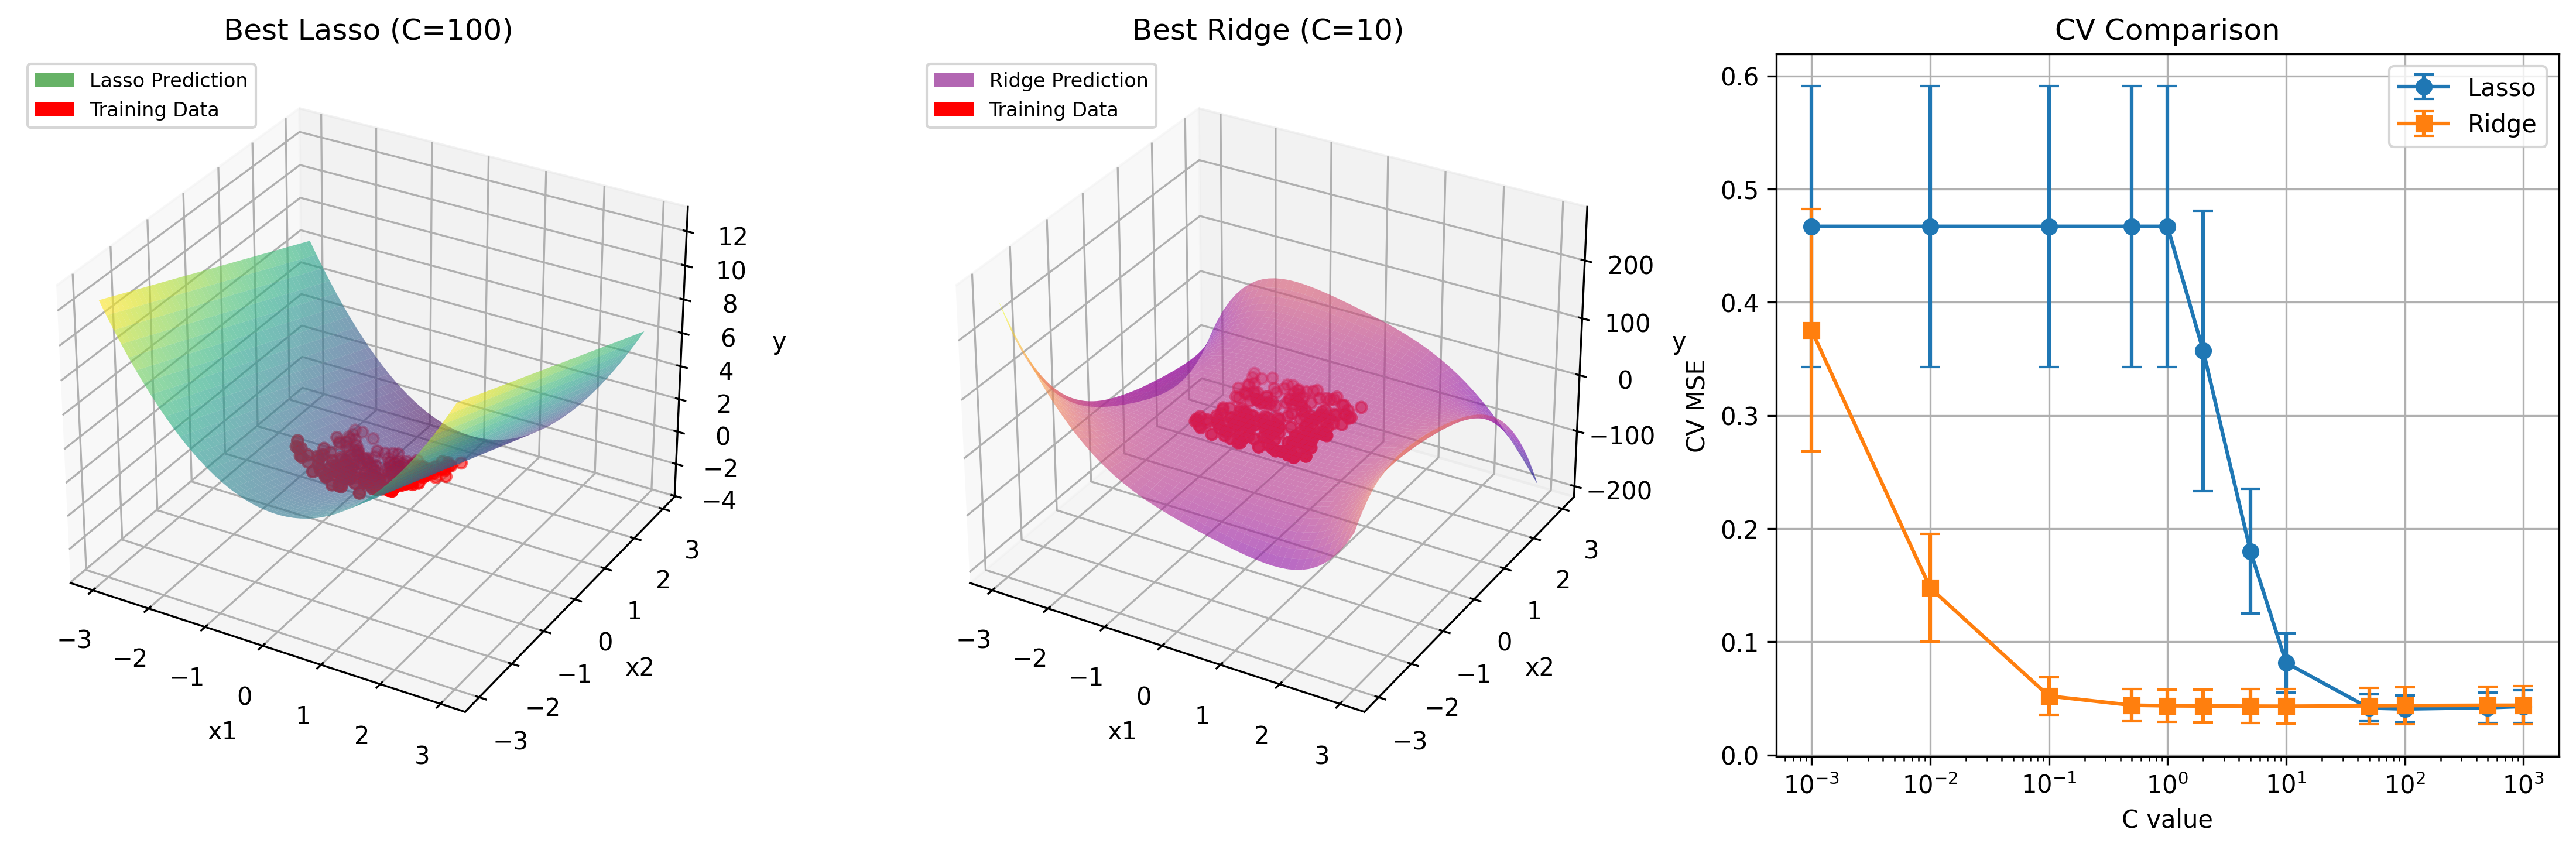
\includegraphics[width=\textwidth]{figures/08_final_comparison.png}
\caption{Final comparison: Left - Best Lasso model (C=100) with 2 features. Center - Best Ridge model (C=10) with all 21 features. Right - CV performance comparison showing both models achieve similar error rates.}
\label{fig:final_comparison}
\end{figure}

\section*{APPENDIX}

\begin{lstlisting}
import numpy as np
import matplotlib.pyplot as plt
from mpl_toolkits.mplot3d import Axes3D
from sklearn.preprocessing import PolynomialFeatures
from sklearn.linear_model import Lasso, Ridge
from sklearn.model_selection import KFold
from sklearn.metrics import mean_squared_error
from matplotlib.patches import Patch

data = np.loadtxt('week3.csv', delimiter=',', skiprows=1)
X = data[:, :2]
y = data[:, 2]
print('data shapes:', X.shape, y.shape)
poly = PolynomialFeatures(degree=5, include_bias=True)
Xpoly = poly.fit_transform(X)

def C_to_alpha(C):
    return 1.0/(2.0*C)

C_list = [0.1, 1, 10]
lasso_results = []
for C in C_list:
    model = Lasso(alpha=C_to_alpha(C), max_iter=10000)
    model.fit(Xpoly, y)
    pred = model.predict(Xpoly)
    mse = mean_squared_error(y, pred)
    lasso_results.append((C, mse, model))

ridge_results = []
for C in C_list:
    model = Ridge(alpha=C_to_alpha(C))
    model.fit(Xpoly, y)
    pred = model.predict(Xpoly)
    mse = mean_squared_error(y, pred)
    ridge_results.append((C, mse, model))

print('Lasso (C, MSE):', [(c, round(m,4)) for c,m,_ in lasso_results])
print('Ridge (C, MSE):', [(c, round(m,4)) for c,m,_ in ridge_results])

# Best lasso
best_C, best_mse, best_model = sorted(lasso_results, key=lambda t: t[1])[0]
print('best lasso C:', best_C, 'MSE:', round(best_mse,4))

# extend grid beyond data range
x1_range = X[:,0].max() - X[:,0].min()
x2_range = X[:,1].max() - X[:,1].min()
x1_min = X[:,0].min() - 1.0*x1_range
x1_max = X[:,0].max() + 1.0*x1_range
x2_min = X[:,1].min() - 1.0*x2_range
x2_max = X[:,1].max() + 1.0*x2_range

xx = np.linspace(x1_min, x1_max, 50)
yy = np.linspace(x2_min, x2_max, 50)
X1g, X2g = np.meshgrid(xx, yy)
Xg = np.c_[X1g.ravel(), X2g.ravel()]
Xg_poly = poly.transform(Xg)
Z = best_model.predict(Xg_poly).reshape(X1g.shape)

fig = plt.figure(figsize=(9,7))
ax = fig.add_subplot(111, projection='3d')
ax.plot_surface(X1g, X2g, Z, alpha=0.6, cmap='viridis', edgecolor='none')
ax.scatter(X[:,0], X[:,1], y, s=30, c='r', alpha=0.8, edgecolors='darkred', linewidths=0.5)
ax.set_title(f'Lasso surface (C={best_C})', fontsize=12, pad=15)
ax.set_xlabel('x1', fontsize=10, labelpad=10)
ax.set_ylabel('x2', fontsize=10, labelpad=10)
ax.set_zlabel('y', fontsize=10, labelpad=10)
ax.view_init(elev=20, azim=45)
ax.grid(True, alpha=0.3)
plt.savefig('figures/01_simple_lasso_surface.png', dpi=300, bbox_inches='tight')
plt.show()

kf = KFold(n_splits=5, shuffle=True, random_state=0)
C_try = [0.1, 1, 10]
cv_means = []
cv_stds = []

for C in C_try:
    mses = []
    for train_idx, test_idx in kf.split(Xpoly):
        model = Lasso(alpha=C_to_alpha(C), max_iter=10000)
        model.fit(Xpoly[train_idx], y[train_idx])
        pred = model.predict(Xpoly[test_idx])
        mses.append(mean_squared_error(y[test_idx], pred))
    cv_means.append(np.mean(mses))
    cv_stds.append(np.std(mses))

print('CV Lasso (C, mean MSE, std):')
for i, C in enumerate(C_try):
    print(C, round(cv_means[i],4), round(cv_stds[i],4))

# (i)(a): 3D scatter plot
fig = plt.figure(figsize=(10,7))
ax = fig.add_subplot(111, projection='3d')
scatter = ax.scatter(X[:,0], X[:,1], y, c=y, cmap='viridis', s=30)

ax.set_xlabel('Feature 1 (x1)')
ax.set_ylabel('Feature 2 (x2)')
ax.set_zlabel('Target (y)')
ax.set_title('3D Scatter Plot')
plt.colorbar(scatter, ax=ax, shrink=0.5, aspect=5, label='Target (y)')

plt.savefig('figures/02_3d_scatter_plot.png', dpi=300, bbox_inches='tight')
plt.show()

# (i)(b): Lasso with polynomial features up to power 5
print("Polynomial features shape:", Xpoly.shape)

C_values = [0.001, 0.01, 0.1, 1, 10, 100, 1000]
lasso_models = {}

print("\nLasso Results:")
print("C\t\tNon-zero coeffs\tMSE")
print("-" * 40)
for C in C_values:
    model = Lasso(alpha=C_to_alpha(C), max_iter=10000)
    model.fit(Xpoly, y)    
    pred = model.predict(Xpoly)
    mse = mean_squared_error(y, pred)
    non_zero = np.sum(np.abs(model.coef_) > 1e-10)
    
    lasso_models[C] = model
    print(f"{C}\t\t{non_zero}\t\t{mse:.4f}")

feature_names = poly.get_feature_names_out(['x1', 'x2'])
print(f"\nPolynomial features: {len(feature_names)} total")
for i, name in enumerate(feature_names):
    print(f"{i:2d}: {name}")

print("Detailed Lasso Coefficients:")
print("=" * 50)

for C in [0.001, 10, 100, 1000]:
    print(f"\nC = {C}:")
    model = lasso_models[C]
    coeffs = model.coef_
    non_zero_indices = np.where(np.abs(coeffs) > 1e-10)[0]
    
    if len(non_zero_indices) == 0:
        print("  All coefficients are zero")
    else:
        print("  Non-zero coefficients:")
        for idx in non_zero_indices:
            print(f"    {feature_names[idx]}: {coeffs[idx]:.6f}")
    print(f"  Total: {len(non_zero_indices)}/{len(coeffs)}")

# (i)(c): Generate predictions and plot surfaces

xx = np.linspace(x1_min, x1_max, 50)
yy = np.linspace(x2_min, x2_max, 50)
X1, X2 = np.meshgrid(xx, yy)

Xgrid = np.c_[X1.ravel(), X2.ravel()]
Xgrid_poly = poly.transform(Xgrid)

fig = plt.figure(figsize=(15, 10))

C_to_plot = [0.001, 1, 1000]
for i, C in enumerate(C_to_plot):
    model = lasso_models[C]
    ypred = model.predict(Xgrid_poly)
    ypred = ypred.reshape(X1.shape)
    
    ax = fig.add_subplot(2, 3, i+1, projection='3d')
    ax.plot_surface(X1, X2, ypred, alpha=0.6, cmap='viridis')
    ax.scatter(X[:,0], X[:,1], y, c='red', s=20)
    ax.set_title(f'Lasso C={C}')
    ax.set_xlabel('x1')
    ax.set_ylabel('x2')
    ax.set_zlabel('y')
    legend_elements = [Patch(facecolor='green', alpha=0.6, label='Lasso Prediction'),
                       Patch(facecolor='red', label='Training Data')]
    ax.legend(handles=legend_elements, loc='upper left', fontsize=8)

plt.tight_layout()
plt.savefig('figures/03_lasso_prediction_surfaces.png', dpi=300, bbox_inches='tight')
plt.show()

# (i)(d): Analyze underfitting and overfitting
mse_list = []
coeff_count = []

for C in C_values:
    model = lasso_models[C]
    pred = model.predict(Xpoly)
    mse = mean_squared_error(y, pred)
    non_zero = np.sum(np.abs(model.coef_) > 1e-10)
    
    mse_list.append(mse)
    coeff_count.append(non_zero)

fig, (ax1, ax2) = plt.subplots(1, 2, figsize=(12, 5))

ax1.semilogx(C_values, mse_list, 'bo-', label='Training MSE')
ax1.set_xlabel('C value')
ax1.set_ylabel('Training MSE')
ax1.set_title('Training MSE vs C')
ax1.legend(loc='best')
ax1.grid(True)

ax2.semilogx(C_values, coeff_count, 'ro-', label='Non-zero Coefficients')
ax2.set_xlabel('C value')
ax2.set_ylabel('Non-zero Coefficients')
ax2.set_title('Model Complexity vs C')
ax2.legend(loc='best')
ax2.grid(True)

plt.tight_layout()
plt.savefig('figures/04_underfitting_overfitting_analysis.png', dpi=300, bbox_inches='tight')
plt.show()

print("Underfitting and Overfitting Analysis:")
print("=" * 40)
print("Small C (high regularization):")
print(f"  C=0.001: MSE={mse_list[0]:.4f}, Coeffs={coeff_count[0]}")
print("  -> underfitting")

print("\nMedium C:")
print(f"  C=1: MSE={mse_list[3]:.4f}, Coeffs={coeff_count[3]}")

print("\nLarge C (low regularization):")
print(f"  C=1000: MSE={mse_list[6]:.4f}, Coeffs={coeff_count[6]}")
print("  -> possibly overfitting")

# (i)(e): Ridge regression comparison
ridge_models = {}

print("Ridge Results:")
print("C\t\tMSE")
print("-" * 20)

for C in C_values:
    model = Ridge(alpha=C_to_alpha(C))
    model.fit(Xpoly, y)
    
    pred = model.predict(Xpoly)
    mse = mean_squared_error(y, pred)
    
    ridge_models[C] = model
    
    print(f"{C}\t\t{mse:.4f}")

# compare Lasso vs Ridge coefficients for C=1
print("\nCoefficient Comparison (C=1):")
print("=" * 40)
lasso_model = lasso_models[1]
ridge_model = ridge_models[1]

print("Feature\t\t\tLasso\t\tRidge")
print("-" * 50)
for i, name in enumerate(feature_names):
    lasso_val = lasso_model.coef_[i]
    ridge_val = ridge_model.coef_[i]
    if abs(lasso_val) > 1e-10 or abs(ridge_val) > 1e-10:
        print(f"{name:20s}\t{lasso_val:8.4f}\t{ridge_val:8.4f}")

fig = plt.figure(figsize=(15, 5))

C_to_plot = [0.001, 1, 1000]
for i, C in enumerate(C_to_plot):
    model = ridge_models[C]
    ypred = model.predict(Xgrid_poly)
    ypred = ypred.reshape(X1.shape)
    
    ax = fig.add_subplot(1, 3, i+1, projection='3d')
    ax.plot_surface(X1, X2, ypred, alpha=0.6, cmap='plasma')
    ax.scatter(X[:,0], X[:,1], y, c='red', s=20)
    ax.set_title(f'Ridge C={C}')
    ax.set_xlabel('x1')
    ax.set_ylabel('x2')
    ax.set_zlabel('y')
    legend_elements = [Patch(facecolor='purple', alpha=0.6, label='Ridge Prediction'),
                       Patch(facecolor='red', label='Training Data')]
    ax.legend(handles=legend_elements, loc='upper left', fontsize=8)

plt.tight_layout()
plt.savefig('figures/05_ridge_prediction_surfaces.png', dpi=300, bbox_inches='tight')
plt.show()

# (ii)(a): 5-fold cross-validation for Lasso
kf = KFold(n_splits=5, shuffle=True, random_state=42)
C_cv = [0.001, 0.01, 0.1, 0.5, 1, 2, 5, 10, 50, 100, 500, 1000]
cv_means = []
cv_stds = []

print("5-Fold CV Results for Lasso:")
print("C\t\tMean MSE\tStd MSE")
print("-" * 35)

for C in C_cv:
    scores = []
    for train_idx, val_idx in kf.split(Xpoly):
        model = Lasso(alpha=C_to_alpha(C), max_iter=10000)
        model.fit(Xpoly[train_idx], y[train_idx])
        pred = model.predict(Xpoly[val_idx])
        scores.append(mean_squared_error(y[val_idx], pred))
    
    mean_score = np.mean(scores)
    std_score = np.std(scores)
    cv_means.append(mean_score)
    cv_stds.append(std_score)
    
    print(f"{C}\t\t{mean_score:.4f}\t\t{std_score:.4f}")

plt.figure(figsize=(10, 6))
plt.errorbar(C_cv, cv_means, yerr=cv_stds, fmt='o-', capsize=5, label='Mean CV MSE ± Std Dev')
plt.xscale('log')
plt.xlabel('C value')
plt.ylabel('CV MSE')
plt.title('5-Fold Cross-Validation for Lasso')
plt.legend(loc='best')
plt.grid(True)
plt.savefig('figures/06_lasso_cv_results.png', dpi=300, bbox_inches='tight')
plt.show()

# (ii)(b): Find optimal C value
best_idx = np.argmin(cv_means)
best_C = C_cv[best_idx]
best_mse = cv_means[best_idx]
best_std = cv_stds[best_idx]

print(f"Optimal C value: {best_C}")
print(f"Best CV MSE: {best_mse:.4f} ± {best_std:.4f}")

final_lasso = Lasso(alpha=C_to_alpha(best_C), max_iter=10000)
final_lasso.fit(Xpoly, y)

print(f"\nFinal Lasso Model (C={best_C}) Coefficients:")
print("=" * 45)
non_zero_indices = np.where(np.abs(final_lasso.coef_) > 1e-10)[0]
for idx in non_zero_indices:
    print(f"{feature_names[idx]}: {final_lasso.coef_[idx]:.6f}")

print(f"\nTotal non-zero coefficients: {len(non_zero_indices)}/{len(final_lasso.coef_)}")
print(f"\nFinal:")
print(f"- Lowest CV MSE: {best_mse:.4f}")
print(f"- Features selected: {len(non_zero_indices)}")

# (ii)(c): 5-fold cross-validation for Ridge
ridge_cv_means = []
ridge_cv_stds = []

print("5-Fold CV Results for Ridge:")
print("C\t\tMean MSE\tStd MSE")
print("-" * 35)

for C in C_cv:
    scores = []
    for train_idx, val_idx in kf.split(Xpoly):
        model = Ridge(alpha=C_to_alpha(C))
        model.fit(Xpoly[train_idx], y[train_idx])
        pred = model.predict(Xpoly[val_idx])
        scores.append(mean_squared_error(y[val_idx], pred))
    
    mean_score = np.mean(scores)
    std_score = np.std(scores)
    ridge_cv_means.append(mean_score)
    ridge_cv_stds.append(std_score)
    
    print(f"{C}\t\t{mean_score:.4f}\t\t{std_score:.4f}")

plt.figure(figsize=(12, 5))
plt.subplot(1, 2, 1)
plt.errorbar(C_cv, cv_means, yerr=cv_stds, fmt='o-', capsize=5, label='Lasso CV MSE ± Std Dev')
plt.xscale('log')
plt.xlabel('C value')
plt.ylabel('CV MSE')
plt.title('Lasso CV Results')
plt.legend(loc='best')
plt.grid(True)

plt.subplot(1, 2, 2)
plt.errorbar(C_cv, ridge_cv_means, yerr=ridge_cv_stds, fmt='s-', capsize=5, label='Ridge CV MSE ± Std Dev', color='orange')
plt.xscale('log')
plt.xlabel('C value')
plt.ylabel('CV MSE')
plt.title('Ridge CV Results')
plt.legend(loc='best')
plt.grid(True)

plt.tight_layout()
plt.savefig('figures/07_lasso_ridge_cv_comparison.png', dpi=300, bbox_inches='tight')
plt.show()

# find optimal Ridge C
best_ridge_idx = np.argmin(ridge_cv_means)
best_ridge_C = C_cv[best_ridge_idx]
best_ridge_mse = ridge_cv_means[best_ridge_idx]

print(f"\nOptimal Ridge C: {best_ridge_C}")
print(f"Best Ridge CV MSE: {best_ridge_mse:.4f}")

print(f"\nComparison:")
print(f"Best Lasso (C={best_C}): CV MSE = {best_mse:.4f}")
print(f"Best Ridge (C={best_ridge_C}): CV MSE = {best_ridge_mse:.4f}")

if best_mse < best_ridge_mse:
    print("Lasso performs better")
else:
    print("Ridge performs better")

fig = plt.figure(figsize=(15, 5))

# Lasso surface
final_lasso_pred = final_lasso.predict(Xgrid_poly).reshape(X1.shape)
ax1 = fig.add_subplot(1, 3, 1, projection='3d')
ax1.plot_surface(X1, X2, final_lasso_pred, alpha=0.6, cmap='viridis')
ax1.scatter(X[:,0], X[:,1], y, c='red', s=20)
ax1.set_title(f'Best Lasso (C={best_C})')
ax1.set_xlabel('x1')
ax1.set_ylabel('x2')
ax1.set_zlabel('y')
legend_elements = [Patch(facecolor='green', alpha=0.6, label='Lasso Prediction'),
                   Patch(facecolor='red', label='Training Data')]
ax1.legend(handles=legend_elements, loc='upper left', fontsize=8)

# Ridge surface
final_ridge = Ridge(alpha=C_to_alpha(best_ridge_C))
final_ridge.fit(Xpoly, y)
final_ridge_pred = final_ridge.predict(Xgrid_poly).reshape(X1.shape)
ax2 = fig.add_subplot(1, 3, 2, projection='3d')
ax2.plot_surface(X1, X2, final_ridge_pred, alpha=0.6, cmap='plasma')
ax2.scatter(X[:,0], X[:,1], y, c='red', s=20)
ax2.set_title(f'Best Ridge (C={best_ridge_C})')
ax2.set_xlabel('x1')
ax2.set_ylabel('x2')
ax2.set_zlabel('y')
legend_elements = [Patch(facecolor='purple', alpha=0.6, label='Ridge Prediction'),
                   Patch(facecolor='red', label='Training Data')]
ax2.legend(handles=legend_elements, loc='upper left', fontsize=8)

# CV comparison
ax3 = fig.add_subplot(1, 3, 3)
ax3.errorbar(C_cv, cv_means, yerr=cv_stds, fmt='o-', capsize=4, label='Lasso')
ax3.errorbar(C_cv, ridge_cv_means, yerr=ridge_cv_stds, fmt='s-', capsize=4, label='Ridge')
ax3.set_xscale('log')
ax3.set_xlabel('C value')
ax3.set_ylabel('CV MSE')
ax3.set_title('CV Comparison')
ax3.legend()
ax3.grid(True)
plt.tight_layout()
plt.savefig('figures/08_final_comparison.png', dpi=300, bbox_inches='tight')
plt.show()
\end{lstlisting} 

\end{document}

